%% ---------------------------------------------------------------------
%% Document class
%% ---------------------------------------------------------------------
\documentclass[11pt]{article}

%% ---------------------------------------------------------------------
%% Packages 
%% ---------------------------------------------------------------------
\usepackage{mathptmx}
\usepackage{graphicx}
\usepackage{times}
\usepackage{amssymb}
\usepackage{parskip}
\usepackage{wrapfig}

%% ---------------------------------------------------------------------
%% Document data
%% ---------------------------------------------------------------------
\title{ECE 264 -- Spring 2013\\ Huffman Coding}
\author{(Derived from an assignment by Professor Vijay Raghunathan)}
\date{}

%% ---------------------------------------------------------------------
%% Document Beginning
%% ---------------------------------------------------------------------
\begin{document}

\maketitle

Huffman coding is a widely used compression algorithm used in JPEG
compression as well as in MP3 audio compression.  This document
explains the technique.  Please see the respective SPEC files for PA10
and PA11 for concrete details on what to do.

\section{ASCII Coding}

Many programming languages use ASCII (which stands for American
Standard Code for Information Interchange) encoding to represent
characters.  In ASCII encoding, every character is encoded
(represented) with the same number of bits (8-bits) per character.
Since there are 256 different values that can be represented with
8-bits, there are potentially 256 different characters in the ASCII
character set, as shown in the ASCII character table available at
http://www.asciitable.com/.
 
Let us now look at a simple example of ASCII encoding of characters.
Using ASCII encoding (8 bits per character) the 13-character string
"go go gophers" requires 13 * 8 = 104 bits.  The table below shows how
the coding works.

\begin{tabular}{lll}
  \hline
  \textbf{Character} & \textbf{ASCII Code} & \textbf{8-bit binary value}\\
  \hline
  Space	& 32 & 00100000\\
  e & 101 & 01100101\\
  g & 103 & 01100111\\
  h & 104 & 01101000\\
  o & 111 & 01101111\\
  p & 112 & 01110000\\
  r & 114 & 01110010\\
  s & 115 & 01110011\\
  \hline
\end{tabular}

The given string would be written as the following stream of bits (the
spaces would not be written, just the 0's and 1's)

\begin{verbatim} 
01100111 01101111 00100000 01100111 01101111 00100000
01100111 01101111 01110000 01101000 01100101 01110010
01110011
\end{verbatim}

\section{From ASCII Coding Towards Huffman Coding}

Next, let us see how we might use fewer bits using a simpler coding
scheme.  Since there are only 8 different characters in "go go
gophers", it is possible to use only 3-bits to encode the 8 different
characters.  We might, for example, use the coding shown in the table
below (keep in mind that other 3-bit encodings are also possible).

\begin{tabular}{lll}
  \hline
  \textbf{Character} & \textbf{Code Value} & \textbf{3-bit binary value}\\
  \hline
  g & 0	& 000\\
  o & 1 & 001\\
  p & 2 & 010\\
  h & 3 & 011\\
  e & 4 & 100\\
  r & 5 & 101\\
  s & 6 & 110\\
  Space & 7 & 111\\
  \hline
\end{tabular}

Now the string "go go gophers" would be encoded as: \texttt{000 001
  111 000 001 111 000 001 010 011 100 101 110}.  As you can see, by
using three bits per character instead of eight bits per character
that ASCII uses, the string "go go gophers" uses a total of 39 bits
instead of 104 bits.
 
However, even in this improved coding scheme, we used the same number
of bits to represent each character, irrespective of how often the
character appears in our string.  Even more bits can be saved if we
use fewer than three bits to encode characters like g, o, and space
that occur frequently and more than three bits to encode characters
like e, h, p, r, and s that occur less frequently in "go go gophers".
This is the basic idea behind Huffman coding: to use fewer bits for
characters that occur more frequently.  We will see how this is done
using a tree data structure that stores the characters as its leaf
nodes, and whose root-to-leaf paths provide the bit sequence used to
encode the characters.

\subsection{Towards a Coding Tree}

Using a binary tree for coding, all characters are stored at the
leaves of a tree.  A left-edge is numbered 0 and a right-edge is
numbered 1.  The code for any character/leaf node is obtained by
following the root-to-leaf path and concatenating the 0's and 1's. The
specific structure of the tree determines the coding of any leaf node
using the 0/1 edge convention described.  As an example, the tree below
yields the coding table following it.

\begin{center}
  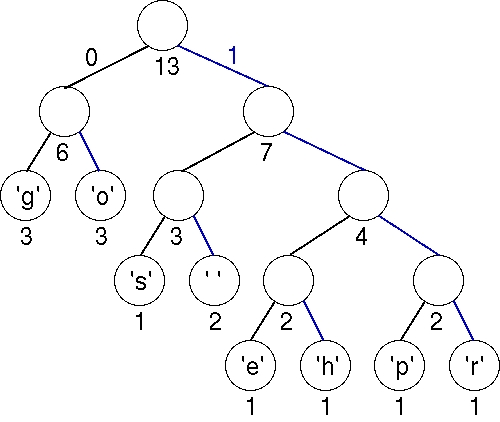
\includegraphics[width=5cm]{figures/ngopher8}
\end{center}

\begin{tabular}{ll}
  \hline
  \textbf{Character} & \textbf{Binary code}\\
  \hline
  ' ' & 101\\
  'e' & 1100\\
  'g' & 00\\
  'h' & 1101\\
  'o' & 01\\
  'p' & 1110\\
  'r' & 1111\\
  's' & 100\\
  \hline
\end{tabular}

Using this coding, "go go gophers" is encoded (again, spaces would not
appear in the bit-stream) as: \texttt{00 01 101 00 01 101 00 01 1110
  1101 1100 1111 100}.  This is a total of 37 bits, two bits fewer
than the improved encoding in which each of the 8 characters has a
3-bit encoding!  The bits are saved by coding frequently occurring
characters like 'g' and 'o' with fewer bits (here two bits) than
characters that occur less frequently like 'p', 'h', 'e', and 'r'.
 
To decode a given stream that has been coded by the given tree, start
at the root of the tree, and follow a left-branch if the next bit in
the stream is a 0, and a right branch if the next bit in the stream is
a 1.  When you reach a leaf, write the character stored at the leaf,
and start again at the top of the tree.  The bit stream
\texttt{10011101101110011111100} yields right-left-left to the letter
's', followed (starting again at the root) with right-right-right-left
to the letter 'p', followed by right-right-left-right to the letter
'h'.  Continuing thus yields a decoded string "sphere."

\subsection{Prefix codes}
 
When all characters are stored in leaves, and every interior
(non-leaf) node has two children, the coding induced by the 0/1
convention outlined above satisfies a very important property called
the \textit{prefix property} which states that no bit-sequence
encoding of a character is the prefix of the bit-sequence encoding of
any other character.  This makes it possible to decode a bitstream
using the coding tree by following root-to-leaf paths.  The tree shown
above for "go go gophers" satisfies this prefix property and is an
optimal tree.  There are other trees that use 37 bits; for example you
can simply swap any sibling nodes and get a different encoding that
uses the same number of bits.  Next, we look at an algorithm for
constructing such an optimal tree.  This algorithm is called Huffman
coding, and was invented by David A. Huffman in 1952 when he was a
Ph.D. student at MIT.

\section{Huffman Coding}

In the previous section we saw examples of how a stream of bits can be
generated from an encoding.  We also saw how the tree can be used to
decode a stream of bits.  We will discuss how to construct the tree
here using Huffman's algorithm.

We will assume that associated with each character is a weight that is
equal to the number of times the character occurs in a file.  For
example, in the string "go go gophers", the characters 'g' and 'o'
have weight 3, the space has weight 2, and the other characters have
weight 1.  When compressing a file, we will need to first read the
file and calculate these weights.  Assume that all the character
weights have been calculated.  Huffman's algorithm assumes that we are
building a single tree from a group (or forest) of trees.  Initially,
all the trees have a single node containing a character and the
character's weight.  Iteratively, a new tree is formed by picking two
trees and making a new tree whose child nodes are the roots of the two
trees.  The weight of the new tree is the sum of the weights of the
two sub-trees.  This decreases the number of trees by one in each
iteration.  The process iterates until there is only one tree
left. The algorithm is as follows:

\begin{enumerate}

\item Begin with a forest of trees.  All trees have just one node,
  with the weight of the tree equal to the weight of the character in
  the node.  Characters that occur most frequently have the highest
  weights. Characters that occur least frequently have the smallest
  weights.

\item Repeat this step until there is only one tree: 
  
  Choose two trees with the smallest weights; call these trees T1 and
  T2. Create a new tree whose root has a weight equal to the sum of
  the weights T1 + T2 and whose left sub-tree is T1 and whose right
  sub-tree is T2.

\item The single tree left after the previous step is an optimal
  encoding tree.

\end{enumerate} 

We shall use the string "go go gophers" as an example.  Initially we
have the forest shown below.  The nodes are shown with a weight that
represents the number of times the node's character occurs in the
given input string/file.

\begin{center}
  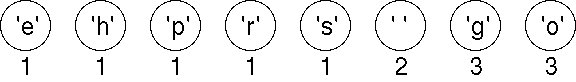
\includegraphics[width=5cm]{figures/ngopher1}
\end{center}

We pick two minimal nodes. There are five nodes with the minimal
weight of 1.  In this implementation, we maintain a priority queue
with items arranged according to their weights.  When two items have
the same weight, a leaf node (i.e., a node associated with an ASCII
character) is always ordered first.  If both nodes are leaf nodes,
they are ordered according to their ASCII coding.  If both nodes are
non-leaf nodes, they are ordered according to the creation times of
the nodes.  We always pick the first two items in the priority queue,
namely, nodes for characters 'e' and 'h'.  We create a new tree whose
root is weighted by the sum of the weights chosen.  The order of the
nodes in the priority queue also determines the left and right child
nodes of the new root.  We now have a forest of seven trees as shown
here.  Although the newly created node has the same weight as Space,
it is ordered after Space in the priority queue because Space is an
ASCII character.

\begin{center}
  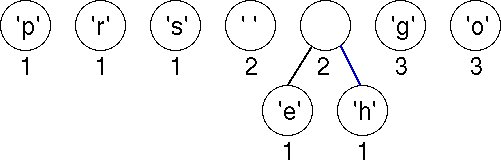
\includegraphics[width=5cm]{figures/ngopher2}
\end{center}

Choosing the first two (minimal) nodes in the priority queue yields
another tree with weight 2 as shown below.  There are now six trees in
the forest of trees that will eventually build an encoding tree.

\begin{center}
  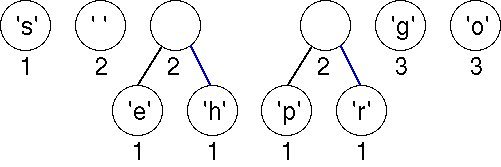
\includegraphics[width=5cm]{figures/ngopher3}
\end{center}

Again we must choose the first two (minimal) nodes in the priority
queue.  The lowest weight is the 'e'-node/tree with weight equal to 1.
There are three trees with weight 2; the one chosen corresponds to an
ASCII character because of the way we order the nodes in the priority
queue.  The new tree has a weight of 3, which will be placed last in
the priority queue according to our ordering strategy.

\begin{center}
  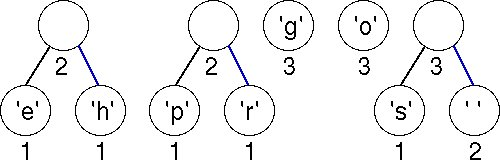
\includegraphics[width=5cm]{figures/ngopher4}
\end{center}

Now there are two trees with weight equal to 2.  These are joined into
a new tree whose weight is 4.  There are four trees left, one whose
weight is 4 and three with a weight of 3.

\begin{center}
  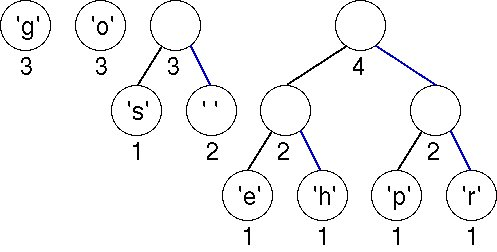
\includegraphics[width=5cm]{figures/ngopher5}
\end{center}

The first two minimal (weight 3) trees in the priority queue are
joined into a tree whose weight is 6.  There are three trees left.

\begin{center}
  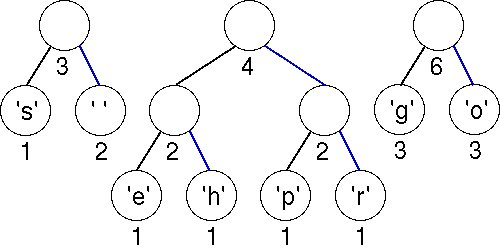
\includegraphics[width=5cm]{figures/ngopher6}
\end{center}

The minimal trees have weights of 3 and 4; these are joined into a
tree with weight 7.

\begin{center}
  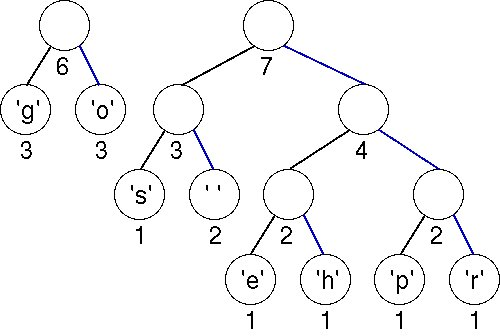
\includegraphics[width=5cm]{figures/ngopher7}
\end{center}

Finally, the last two trees are joined into a final tree whose weight
is 13, the sum of the two weights 6 and 7.  This tree is the tree we
used to illustrate Huffman coding above.  Note that you can easily
come up with an alternative optimal tree by using a different ordering
strategy to order trees of the same weights.  In that case, the bit
patterns for each character are different, but the total number of
bits used to encode "go go gophers" is the same.

\begin{center}
  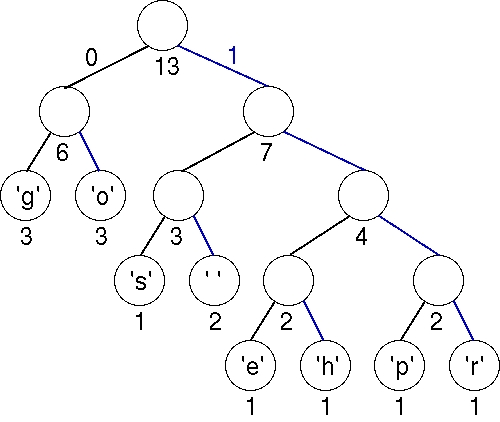
\includegraphics[width=5cm]{figures/ngopher8}
\end{center}

We now show another tree to compress the string "streets are stone
stars are not" optimally.  To encode "streets are" we would have the
following bits:

\texttt{1110001111011000111101010011110}.

\begin{center}
  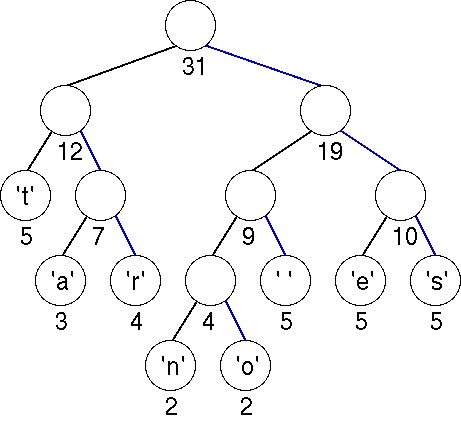
\includegraphics[width=5cm]{figures/streetstar}
\end{center}

\begin{tabular}{ll}
  \hline
  \textbf{Character} & \textbf{Binary code}\\
  \hline
  '  ' & 101\\
  'a' & 010\\
  'e' & 110\\
  'n' & 1000\\
  'o' & 1001\\
  'r' & 011\\
  's' & 111\\
  't' & 00\\
  \hline
\end{tabular}

It is important to note that you cannot use the tree built for the
string "go go gophers" to decode the bitstreams obtained from the
encoding of "streets are stone stars are not" as the encoding is
performed using a different tree.

\section{Reading Huffman Headers}
 
You must store some initial information in the compressed file that
will be used by the decompression/unhuffing program.  Basically, you
must store the tree that is used to compress the original file.  This
is because the decompression program needs this exact same tree in
order to decode the data.  The header information contains:

\begin{itemize}

\item The topology of the Huffman coding tree.  To store the tree at
  the beginning of the file, we use a post-order traversal, writing
  each node visited.  When you encounter a leaf node, you write a 1
  followed by the ASCII character of the leaf node.  When you
  encounter a non-leaf node, you write a 0.  To indicate the end of
  the Huffman coding tree, we write another 0.

\item The total number of characters in the input file, followed by a
  newline character.

\end{itemize}
 
Consider the string "go go gophers", the header information is\\
\texttt{"1g1o01s1 01e1h01p1r0000013$\backslash$n"}, where
\texttt{"$\backslash$n"} is the newline character.  The post-order
traversal of the Huffman coding tree gives us \texttt{"1g1o01s1
  01e1h01p1r0000"}. Another \texttt{"0"} separates the topology from
\texttt{"13"}, which is the number of characters in the input file.
 
For the string "streets are stone stars are not", the header
information is\\ \texttt{"1t1a1r001n1o01 01e1s000031$\backslash$n"}.
The resulting tree looks like this:

\begin{center}
  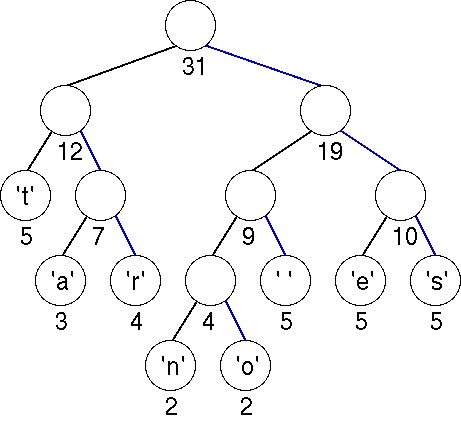
\includegraphics[width=5cm]{figures/streetstar}
\end{center}

The numbers below each leaf node corresponds to the number of
instances each characters appears in the file.  For assignment PA10,
you do not need to worry about this.
 
In these two examples, we use characters 0 and 1 to distinguish
between non-leaf and leaf nodes (and 0 to indicate the end of a
topology).  As there are eight leaf nodes in each of the two examples,
there are eight 1's, seven 0's for non-leaf nodes, and another one 0
to indicate that we have reached the end of a topology.  This approach
used a total of 24 bytes.

To construct a Huffman coding tree from the header information, we
make use of a stack.  When a 1 is read, we read the corresponding
ASCII character and push a node containing the character onto the
stack.  When a 0 is read, if the stack contains only one element, we
have constructed the entire Huffman coding tree.  Otherwise, there
must be more than one element in the stack.  We create a new node, and
pop the top two elements off the stack.  We make the first element off
the stack the right child of the new node, and the second element off
the stack the left child of the new node.  After that, we push the
newly created node onto the stack.
   
\end{document}
